\chapter{Introduction}

\section{Basic Concepts} \label{sec:basic_concepts}

\textbf{\textit{High Performance Computing}} (HPC), also known as \textbf{\textit{supercomputing}}, refers to computing systems with extremely high computational power that are able to solve hugely complex and demanding problems. \cite{europaHighPerformance}

Often, high precision and accuracy are required in scientific and engineering simulations, which can be achieved by increasing the computational power of the system. This is where HPC comes into play, as it allows for the execution of large-scale \textbf{simulations} of complex problems in a reasonable amount of time. Simulations have become the key method for researching and developing innovative solutions in both scientific and engineering fields. They are especially prominent in leading domains such as the aerospace industry and astrophysics, where they enable the investigation and resolution of highly complex problems. However, the increasing reliance on simulation also introduces significant \textbf{challenges related to complexity, scalability, and data management}, which in turn impact the supporting IT infrastructure.

As scientific inquiry progresses along what is known as the \textit{Inference Spiral of System Science}, the complexity of models intensifies and the influx of new data enriches these systems with additional insights. Consequently, this dynamic evolution necessitates ever increasing computational power to efficiently handle the enhanced simulations and data management challenges.

\begin{minipage}[H]{0.6\textwidth}
    \begin{figure}[H]
        \centering
        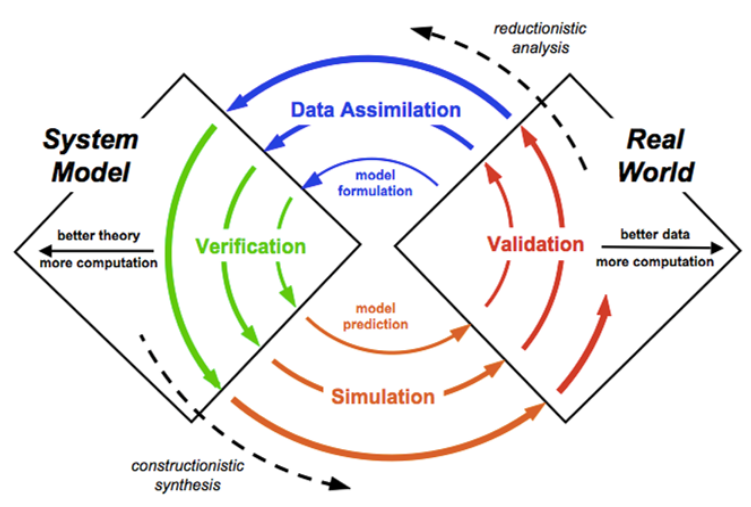
\includegraphics[width=0.85\textwidth]{assets/research.png}
        \caption{Research and Development}
        \label{fig:research}
    \end{figure}
\end{minipage}%
\begin{minipage}[H]{0.4\textwidth}
    \begin{table}[H]
        \centering
        \renewcommand{\arraystretch}{1.15}
        \begin{tabular}{lcc}
            \hline
            \textbf{Prefix} & \textbf{Symbol} & \textbf{Value} \\
            \hline
            Yotta & Y & $10^{24}$ \\
            Zetta & Z & $10^{21}$ \\
            Exa & E & $10^{18}$ \\
            Peta & P & $10^{15}$ \\
            Tera & T & $10^{12}$ \\
            Giga & G & $10^9$ \\
            Mega & M & $10^6$ \\
            Kilo & K & $10^3$ \\
            \hline
        \end{tabular}
        \caption{Prefixes in HPC}
    \end{table}
\end{minipage}

\begin{observationblock}
In today’s world, larger and larger amounts of data are constantly being generated, from 33 zettabytes globally in 2018 to an expected 181 zettabytes in 2025. This exponential growth is driving a shift towards data-intensive applications, making HPC indispensable for processing and analyzing these vast datasets efficiently. Consequently, HPC is key to unlocking valuable insights that benefit citizens, businesses, researchers, and public administrations. \cite{europaHighPerformance}
\end{observationblock}

\subsection{What is High Performance Computing?} \label{sec:what_is_hpc}

High Performance Computing (HPC) involves using powerful \textcolor{red}{servers, clusters, and supercomputers}, along with \textcolor{blue}{specialized software, tools, components, storage, and services}, to solve computationally intensive \textcolor{ForestGreen}{scientific, engineering, or analytical tasks}. 

HPC is used by scientists and engineers both in research and in production across \textcolor{red}{industry}, \textcolor{blue}{government} and \textcolor{ForestGreen}{academia}.

Key elements of the HPC ecosystem include:
\begin{itemize}
    \item \textbf{\textcolor{red}{Hardware}:} High-performance servers, clusters, and supercomputers.
    \item \textbf{\textcolor{blue}{Software}:} Specialized tools and applications designed to optimize complex computations.
    \item \textbf{\textcolor{ForestGreen}{Applications}:} Scientific, engineering, and analytical tasks that leverage high computational power.
\end{itemize}

\textbf{People in HPC}

Human capital is by far the most important aspect in the HPC landscape. Two crucial roles include HPC providers, who plan, install, and manage the resources, and HPC users, who leverage these resources to their fullest potential. The mixing and interplaying of these roles not only enhances individual competence but also drives overall advancements in high-performance computing.

\subsection{Performance and metrics} \label{sec:performance}

\textbf{Performance} in the realm of high-performance computing is a multifaceted concept that extends far beyond a mere measure of speed. While terms such as “how fast” something operates are often used to describe performance, they tend to be vague. Many factors contribute to the overall performance of a system, and the interpretation of these factors can vary depending on the specific context and objectives of the computational task. Performance, therefore, remains a complex and central issue in the field of HPC, as it involves more than just the raw computational speed.

The discussion often extends to the idea that the "P" in HPC might stand for more than just performance. A growing sentiment among professionals in the field suggests that high performance should be complemented by high productivity. This broader view recognizes that the true efficiency of a computing system is not only determined by its ability to perform tasks quickly but also by the ease and speed with which applications can be developed and maintained. In other words, while raw performance is critical, the overall productivity of a system—combining the system's speed with the programmer's effort—plays an equally important role.

To further clarify the distinction, consider that performance can be seen as a measure of how effectively a system executes tasks, whereas productivity is the outcome achieved relative to the effort invested in developing the application. For instance, if a code optimization leads to a system that runs twice as fast but requires an extensive period of development—say, six months of work—the benefits of the improvement must be weighed against the increased effort required. This example underlines the importance of balancing performance gains with the associated development costs.

Ultimately, the challenge lies in understanding and optimizing both aspects. A successful HPC system is one that not only achieves high computational throughput but also enhances the productivity of the developers who create and refine the applications. This balance is essential for advancing the capabilities of high-performance computing in both research and production environments.

\subsubsection{Number Crunching on CPU} \label{sec:number_crunching}

When evaluating the performance of a high-performance computing (HPC) system, one of the most fundamental metrics is the rate at which floating point operations are executed. This rate is typically expressed in millions (Mflops) or billions (Gflops) of operations per second. In essence, it quantifies how many calculations, such as additions and multiplications, the system is capable of performing every second.

To estimate this capability, we rely on the concept of theoretical peak performance. This value is computed by considering the system’s clock rate, the number of floating point operations that can be executed in a single clock cycle, and the total number of processing cores available. Under ideal conditions, the theoretical peak performance can be expressed as follows:

$$
\text{FLOPS} = \text{clock\_rate} \times \text{Number\_of\_FP\_operations} \times \text{Number\_of\_cores}
$$

This formula provides an upper bound on the computational power of the system. However, it is important to note that this is a best-case scenario estimate and does not always reflect the performance achievable in real applications.

\subsubsection{Sustained (Peak) Performance} \label{sec:sustained}

While the theoretical peak performance offers insight into the maximum potential of an HPC system, the actual performance observed during real-world operations is better captured by the sustained (or peak) performance. In practice, several factors such as memory bandwidth limitations, communication latencies, and input/output overhead can prevent a system from reaching its theoretical maximum.

Sustained performance refers to the effective throughput that an HPC system attains when executing actual workloads. Since it is challenging to exactly measure the number of floating point operations performed by every application, standardized benchmarks are commonly used to assess this performance. One widely recognized benchmark is the HPL Linpack test, which forms the basis for the TOP500 list of supercomputers. This benchmark emphasizes the importance of sustained performance, as it reflects the system’s efficiency and reliability under realistic operational conditions.

Understanding both the theoretical and sustained performance metrics is crucial. While the former provides an idealized estimate of a system's capabilities, the latter offers a more practical perspective, thereby guiding decisions on system improvements and resource allocation in high-performance computing environments.


\dots

\subsection{Moore Law}

Tipically, the Moore Law is stated as: "Performance doubles every 18 months". However, it is actually closer to "The number of transistors per unit cost doubles every 18 months".

The original Moore Law was formulated by Gordon Moore, co-founder of Intel, in 1965. He predicted that:

\begin{definitionblock}
    \textit{"The complexity for minimum component costs has increased at a rate of roughly a factor of two per year. [...] Over the longer term, the rate of increase is a bit more uncertain, although there is no reason to believe it will not remain nearly constant for at least 10 years." \newline
    \phantom{ } \hfill \textasciitilde Gordon Moore, 1965}
\end{definitionblock}

Dennard Scaling: From Moore's Law to performance

\begin{definitionblock}
    \textit{"Power density stays constant as transistors get smaller" \newline
    \phantom{ } \hfill \textasciitilde Robert H. Dennard, 1974}
\end{definitionblock}

The concept of Dennard scaling, named after Robert Dennard, an IBM researcher, is closely related to Moore's Law. Dennard scaling refers to the observation that as transistors shrink in size, their power density remains constant. This phenomenon allowed for the continuous increase in clock speeds and performance of microprocessors over the years. 

However, Dennard scaling began to break down around the early 2000s, as power consumption and heat dissipation became significant challenges. Consequently, the industry shifted its focus from increasing clock speeds to improving parallelism and energy efficiency.

\vspace{0.5em}

Intuitively:

\begin{itemize}
    \item Smaller transistors $\rightarrow$ shorter propagation delay $\rightarrow$ faster frequency 
    \item  Smaller transistors $\rightarrow$ smaller capacitance $\rightarrow$ lower power consumption
\end{itemize}

$$
Power \propto Capacitance \times Voltage^2 \times Frequency
$$

\subsubsection{End of Dennard Scaling: Power wall}

The power wall is a fundamental limit on the amount of power that can be dissipated by a chip. This limit is determined by the chip's thermal design power (TDP), which is the maximum amount of heat that the cooling system can dissipate. As the number of transistors on a chip increases, the power consumed by the chip also increases, eventually reaching the TDP limit. When this limit is reached, the chip can no longer dissipate the heat generated by the transistors, leading to overheating and reduced performance.

However, the original Moore's Law is still valid, as the number of transistors per unit cost continues to double every 18 months, but no more on a single core. Instead, the industry has shifted towards multi-core processors and parallel computing to continue improving performance.

\begin{figure}[H]
    \centering
    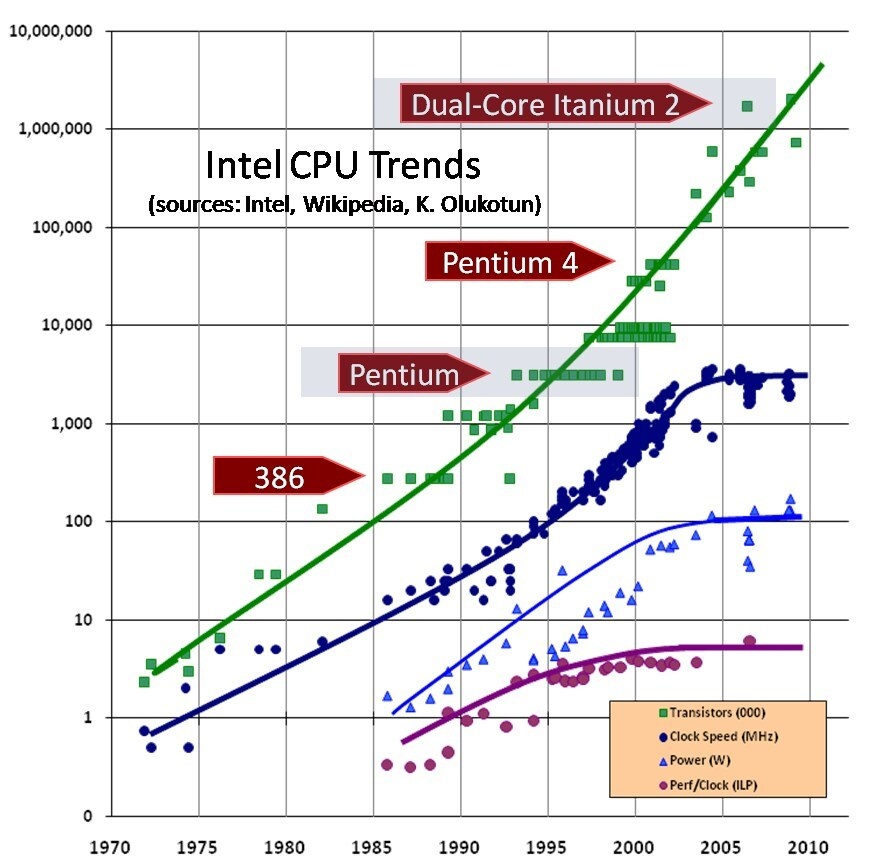
\includegraphics[width=0.6\textwidth]{assets/moore.jpg}
    \caption{Moore's Law}
    \label{fig:moore}
\end{figure}

This evolution marks what many computer scientists and engineers refer to as the end of the "free lunch" era, which began around 2006. Prior to this shift, software developers could rely on hardware improvements to automatically enhance their applications' performance without significant code optimization. Single-core performance scaling, which had been the primary driver of computational advances for decades, effectively plateaued as the industry encountered fundamental physical limitations.

The computing community has responded to this challenge through two complementary approaches:

\textbf{The Software Solution:} This approach emphasizes the critical importance of efficient software design and implementation. As hardware improvements no longer automatically translate to performance gains, developers must engage in deliberate "performance engineering"—applying sophisticated optimization techniques informed by deep understanding of hardware architecture. This involves careful algorithm selection, memory access pattern optimization, and exploitation of instruction-level parallelism to maximize the utilization of available hardware resources.

\textbf{The Specialized Architectural Solution:} The second approach acknowledges a fundamental shift in design constraints: while chip space has become relatively inexpensive, power consumption has emerged as the primary limiting factor. Rather than continuing to develop increasingly complex general-purpose processing cores, this approach advocates for heterogeneous computing systems. Such systems incorporate specialized accelerators (such as GPUs, TPUs, and FPGAs) that are optimized for specific computational patterns. This architectural diversification allows for significant performance improvements in targeted application domains while maintaining reasonable power consumption profiles.

These complementary strategies represent the computing industry's response to the physical limitations that have constrained traditional performance scaling. By combining software optimization with hardware specialization, the field continues to advance computational capabilities even as the straightforward scaling of single-core performance has reached its practical limits.

\subsection{The Shift to Multicore Architecture}

Modern CPUs have evolved into multicore processors due to physical constraints in power consumption and heat dissipation, with manufacturers reducing clock frequencies while increasing core count to deliver greater computational throughput within manageable thermal profiles. These independent cores can execute separate instruction streams simultaneously but share critical resources including memory hierarchies, controllers, and peripheral subsystems, creating a complex environment where cores must cooperate and compete for resources. This architectural shift effectively circumvents the limitations of traditional single-core scaling but presents new challenges for software developers, who must now explicitly design for parallelism to fully leverage available computational capabilities.

[Hardware accelerators image]

\subsection{Parallel Compuers}

Parallel computing is a type of computation in which many calculations or processes are carried out simultaneously. Flynn Taxonomy is a classification of parallel computer architectures, proposed by Michael J. Flynn in 1966. It categorizes computer systems based on the number of instruction streams and data streams that can be processed concurrently. The four categories are shown in Table \ref{tab:hw-sw-comparison}.

\begin{table}[ht]
    \centering
    \begin{tabular}{l p{6.8cm} p{6.8cm}}
        \hline
        \textbf{} & \textbf{HW level} & \textbf{SW level} \\
        \hline
        \textbf{SISD} & 
        A Von Neumann CPU & 
        no parallelism at all \\
        \hline
        \textbf{MISD} & 
        On a superscalar CPU, different ports executing different \textit{read} on the same data & 
        ILP on same data; multiple tasks or threads operating on the same data \\
        \hline
        \textbf{SIMD} & 
        Any vector-capable hardware (vector registers on a core, a GPU, a vector processor, an FPGA, ...) & 
        data parallelism through vector instructions and operations \\
        \hline
        \textbf{MIMD} & 
        Every multi-core processor; on a superscalar CPU, different ports executing different ops on different data & 
        ILP on different data; multiple tasks or threads with different data on each core \\
        \hline
    \end{tabular}
    \caption{Comparison of SISD, MISD, SIMD, and MIMD at HW and SW levels}
    \label{tab:hw-sw-comparison}
\end{table}

While Flynn's taxonomy provided a foundational classification system in 1966, its utility for categorizing modern HPC infrastructure has diminished significantly. The dramatic evolution of CPUs and computing architectures over the past six decades has produced systems with hybrid designs that transcend these simple classifications. Nevertheless, the fundamental concepts of SIMD and MIMD remain relevant principles that continue to influence the design and implementation of contemporary HPC hardware solutions.

\subsection{Essential Components of a HPC Cluster}

\begin{itemize}
    \item Several computers (nodes)
        
        Often in special cases (1U) for easy mounting in racks

    \item One or more networks (interconnects) to hook the nodes together
    \item Some kind of storage
    \item A login/access node
\end{itemize}

[Cluster image]

\section{Single CPU topology}

Modern CPUs are multy- (or many-) core processors.

\begin{definitionblock}
    A \textbf{core} is the smallest unit of computing, having one or more (hardware/software) threads and is responsible for executing instructions.
\end{definitionblock}

A CPU uses a \textbf{Cache hierarchy} to store data and instructions. The cache hierarchy consists of several levels of cache, each with different sizes and access times. The cache hierarchy is designed to minimize the time it takes to access data and instructions, which can significantly improve the performance of the CPU.

[CPU layout image]

% image description

[Node topology image]

% image description

[Overall topology image]

% image description

\dots

\subsection{memory}

on a supercomputer there is a hybrid approach as for the memory placement:

\begin{itemize}
    \item \textbf{Shared memory:} the memory on a single nodes can be accessed directly by all the cores on that node, meaning that memory access is a “read/write” instructions irrespectively of what exact memory bank it refers to.
    \item \textbf{distributed memory:} when you use many nodes at a time, a process can not directly access the memory on a different node. It need to issue a request for that, not a read/write instruction.
\end{itemize}

These are hardware concepts, i.e. they describe how the memory is physically accessible. However, they do also refer to programming paradigms, as we’ll see in a while.


\begin{tipsblock}[Notation]
    \begin{itemize}
        \item \textbf{Multiprocessor:} server with more than 1 CPU
        \item \textbf{Multicore:} CPU with more than 1 core
        \item \textbf{Processor} = CPU = Socket
    \end{itemize}

    Note that sometimes the term “processor” is used to refer to the CPU, sometimes to the core.
\end{tipsblock}

\subsubsection{Shared Memory: UMA}

Uniform memory access (UMA): Each processor has uniform access to memory. Also known as symmetric multiprocessing (SMP).

\begin{figure}[H]
    \centering
    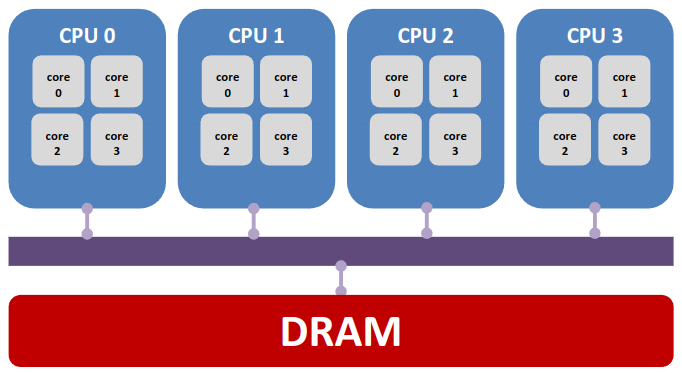
\includegraphics[width=0.6\textwidth]{assets/uma.png}
    \caption{Uniform Memory Access (UMA)}
    \label{fig:uma}
\end{figure}

\subsubsection{Shared memory: NUMA}

Non-uniform memory access (NUMA): Time for memory access depends on location of data. Local access is faster then non-local access.

\begin{figure}[H]
    \centering
    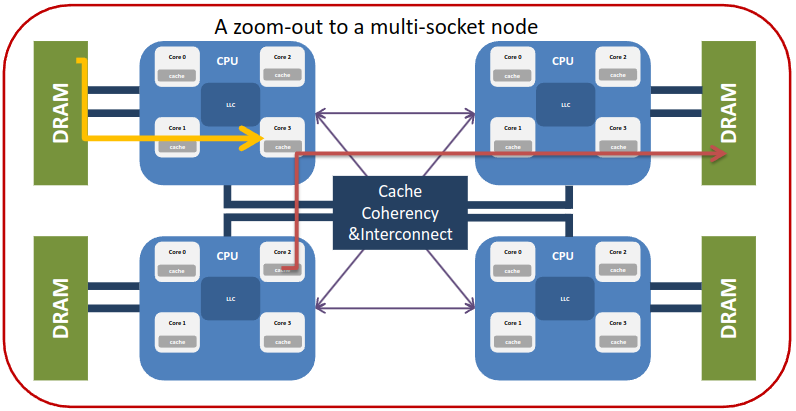
\includegraphics[width=0.6\textwidth]{assets/numa.png}
    \caption{Non-Uniform Memory Access (NUMA)}
    \label{fig:numa}
\end{figure}

\subsubsection{Parallelism within a HPC node}

A single node can have multiple cores, each with multiple hardware threads. This introduces several levels of parallelism:

\begin{figure}[H]
    \centering
    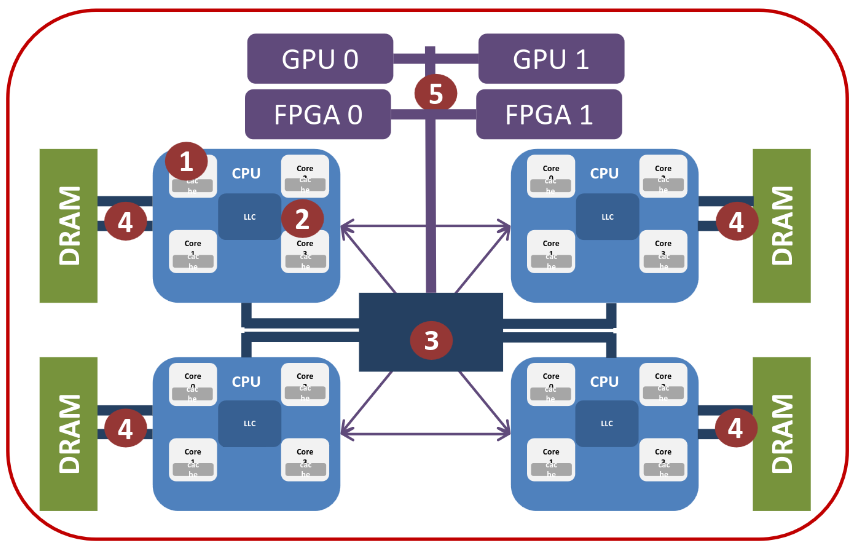
\includegraphics[width=0.6\textwidth]{assets/parallelism.png}
    \caption{Levels of parallelism}
    \label{fig:parallelism}
\end{figure}

\begin{enumerate}
    \item The first level parallelism is in a single core of a CPU
    \item The second level of parallelism is between cores of a single CPU
    \item The third level of parallelism is introduced by inner cache levels
    \item The fourth level of parallelism is between CPUs of a single node.
    \item A node can also have accelerators, like GPUs or FPGAs which introduce another level of parallelism.
\end{enumerate}
